\chapter{A Graph Extension of the Positional Burrows-Wheeler Transform and its Applications}

\section{Abstract}
We present a generalization of the Positional Burrows-Wheeler Transform, or PBWT, to genome graphs, which we call the gPBWT. A genome graph is a collapsed representation of a set of genomes described as a graph. In a genome graph, a haplotype corresponds to a restricted form of walk. The gPBWT is a compressible representation of a set of these graph-encoded haplotypes that allows for efficient subhaplotype match queries. We give efficient algorithms for gPBWT construction and query operations. We describe our implementation, showing the compression and search of 1000~Genomes data.

% I dropped this because we don't really have very structurally interesting variants in the VCF, and VG can't process them anyway. The really cool application is something like MHC with nested variants, but until we get cycles going we can't do it.
% including structural variants that are not handled by the PBWT.
As a demonstration, we use the gPBWT to quickly count the number of haplotypes consistent with random walks in a genome graph, and with the paths taken by mapped reads; results suggest that haplotype consistency information can be practically incorporated into graph-based read mappers. 

\section{Introduction}

The PBWT is a compressible data structure for storing haplotypes that provides an efficient search operation for subhaplotype matches \cite{durbin2014efficient}. Implementations, such as BGT (\url{https://github.com/lh3/bgt}), can be used to compactly store and query thousands of samples. The PBWT can also allow existing haplotype-based algorithms to work on much larger collections of haplotypes than would otherwise be practical \cite{lunter2016fast}. In the PBWT, each site (corresponding to a genetic variant) is a binary feature and the sites are totally ordered. The input haplotypes to the PBWT are binary strings, with each element in the string indicating the state of a site. In the generalization we present, each input haplotype is a walk in a general bidirected graph. This allows haplotypes to be partial (they can start and end at arbitrary nodes) and to traverse arbitrary structural variation. It does not require the sites (nodes in the graph) to have a biologically relevant ordering to provide compression.
% There still has to be *some* ordering of sides for the sorting of visits to work.
However, despite these generalizations, the core data structures are similar, the compression still exploits genetic linkage and the haplotype matching algorithm is essentially the same.

\section{Definitions}

We define $G = (V, E)$ as a \vocab{genome graph} in a bidirected formulation \cite{medvedev2009maximum, paten2014mapping}. Each node in $V$ has a DNA-sequence label; a left, or $5^\prime$, \vocab{side}; and a right, or $3^\prime$, side. Each edge in $E$ is a pairset of sides. The graph is not a multigraph: only one edge may connect a given pair of sides and thus only one \vocab{self-loop} can be present on any given side.

We consider all the sides in the graph to be (arbitrarily) ordered relative to one another. We also define the idea of the \vocab{opposite} of a side $s$, with the notation $\overline{s}$, meaning the side of $s$'s node which is not $s$ (i.e.\ the left side of the node if $s$ is the right side, and the right side of the node if $s$ is the left side). Finally, we use the notation $n(s)$ to denote the node to which a side $s$ belongs.

Within the graph $G$, we define the concept of a \vocab{thread}, which can be used to represent a haplotype or haplotype fragment. A thread $t$ on $G$ is a reversible nonempty sequence of sides, such that for $0 \leq i < N$ sides $t_{2i}$ and $t_{2i+1}$ are opposites of each other, and such that $G$ contains an edge connecting every pair of sides $t_{2i}$ and $t_{2i+1}$. In other words, a thread is a walk through the sides of the graph that alternates traversing nodes and traversing edges and which starts and ends with nodes. Note that a thread is reversible: exactly reversing the sequence of sides making up a thread produces an equivalent thread. We call a thread traversed in a certain direction an \vocab{orientation}. 

We consider $G$ to have associated with it a collection of \vocab{embedded} threads, denoted as $T$. We propose an efficient storage and query mechanism for $T$ given $G$.

% This is where we explain why we are going to do what we are about to do.
Our high-level strategy is to store $T$ by grouping together threads that have recently visited the same sequences of sides, and storing in one place the next sides that those threads will visit. As with the Positional Burrows-Wheeler Transform, used to store haplotypes against a linear reference, and the ordinary Burrows-Wheeler transform, we consider the recent history of a thread to be a strong predictor of where the thread is likely to go next \cite{durbin2014efficient}. By grouping together the next side data such that nearby entries are likely to share values, we can use efficient encodings (such as run-length encodings) and achieve high compression.

More concretely, our approach is as follows. We call an instance of side in a thread a \vocab{visit}; a thread may visit a given side multiple times. Consider all visits of threads in $T$ to a side $s$ where the thread arrives at $s$ either by traversing an edge incident to $s$ (and not by traversing $n(s)$) or by beginning at $s$. For each such visit, take the sequence of sides coming before this arrival at $s$ in the thread and reverse it, and then sort the visits lexicographically by these sequences of sides, breaking ties by an arbitrary global ordering of the threads. Then, for each visit, look two steps ahead in its thread (past $s$ and $\overline{s}$), and note what side comes next (or the null side if the thread ends). After repeating for all the sorted visits to $s$, take all the noted sides in order and produce the array $B_s[]$ for side $s$. An example $B[]$ array and its interpretation are shown in Figure \ref{fig:barray}. (Note that, throughout, arrays are indexed from $0$ and can produce their lengths trivially upon demand.)  

\begin{figure}[h!]
\centering
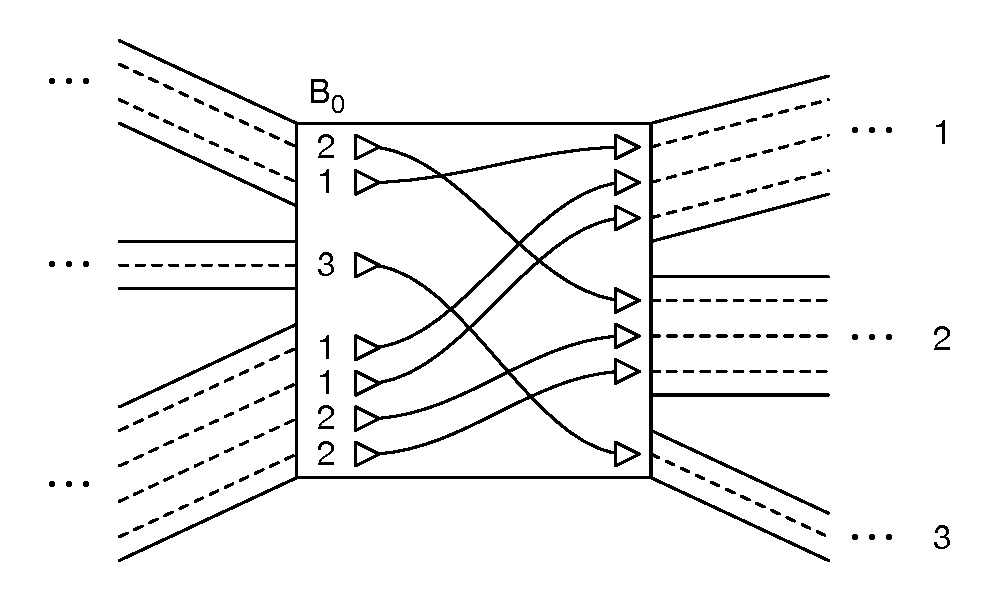
\includegraphics[width=\linewidth]{figures/03_gpbwt/barray.eps}
%Maybe change 0 to s or something.
\caption{An illustration of the $B_{0}[]$ array for a single side numbered $0$. Threads visiting this side may enter their next nodes on sides $1$, $2$, or $3$. The $B_0[]$ array records, for each visit of a thread to side $0$, the side on which it enters its next node. This determines through which of the available edges it should leave the current node. Because threads tend to be similar to each other, they are likely to run in ``ribbons'' of multiple threads that both enter and leave together. These ribbons cause the $B_s[]$ arrays to contain runs of identical values, which may be compressed.}
\label{fig:barray}
\end{figure}

Each unoriented edge $\{ s, s' \}$ in $E$ has two orientations $(s, s')$ and $(s', s)$. Let $c()$ be a function of these oriented edges, such that for an oriented edge $( s, s' )$, $c(s, s')$ is the smallest index in $B_{s'}[]$ of a visit of $s'$ that arrives at $s'$ by traversing $\{ s, s' \}$. Note that, because of the global ordering of sides and the sorting rules defined for $B_{s'}[]$ above, $c(s_0, s')$ will be less than or equal to $c(s_1, s')$ for $s_0 < s_1$ both adjacent to $s'$.

%Since sides are globally ordered, oriented edges, as ordered pairs of sides $(s, s')$, can be globally ordered first by $s$ and then by $s'$. For an edge $\{ s, s' \}$ in $G$, $c(s, s')$ gives the number of traversals, within threads in $T$, of oriented edges ending at $s'$ and ordered before $\{s, s'\}$, plus the number of threads beginning at $s$ without first traversing any edges. This is also, due to the definition of $B[]$ above, the smallest index in $B_{s'}[]$ of a visit of $s'$ that arrives at $s'$ by traversing $\{ s, s' \}$, if any such visit exists.

For a given $G$, we call the combination of the $c()$ function and the $B[]$ arrays a \vocab{graph Positional Burrows Wheeler Transform (gPBWT)}. We submit that a gPBWT is sufficient to represent $T$, and, moreover, that it allows efficient counting of the number of threads in $T$ that contain a given new thread as a subthread. Figure \ref{fig:highwaydiagram} and Table \ref{tbl:barrays} give a worked example.

\begin{figure}[h!]
\centering
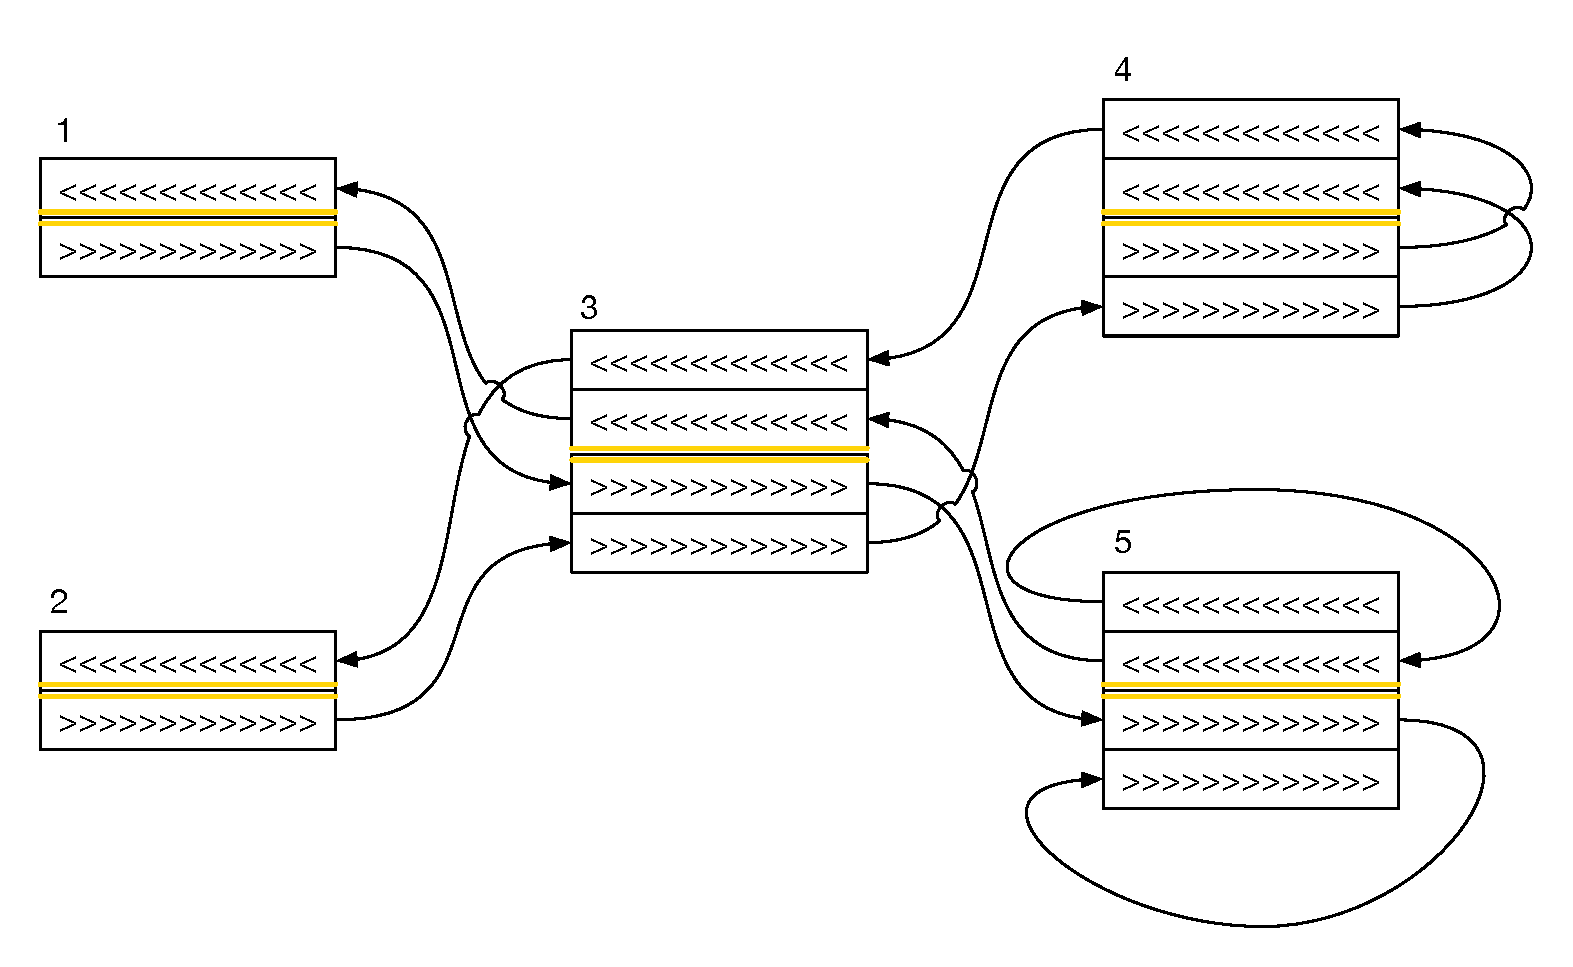
\includegraphics[width=\linewidth]{figures/03_gpbwt/highwaydiagram.eps}
\caption{A diagram of a graph containing two embedded threads. The graph consists of nodes $[1, 2, 3, 4, 5]$, with sides $[1L, 1R, 2L, 2R, \ldots]$, connected by edges $[1R, 3L]$, $[2R, 3L]$, $[3R, 4L]$, $[3R, 5L]$, $[4R, 4R]$, and $[5R, 5L]$. Embedded threads travel on the right-hand side of the nodes they are traveling through. Each thread here corresponds to a pair of ``lanes'' running in opposite directions. Visits are ordered from top to bottom, with ``lanes'' for lesser visits above those for greater ones. the ``lanes'' on the top half of each node are ordered in correspondence with the $B_s[]$ entries for the right side of the node, and those on the bottom half are ordered in correspondence with the $B_s[]$ entries for the left side of the node. The threads shown here are $[1L, 1R, 3L, 3R, 5L, 5R, 5L, 5R]$ and $[2L, 2R, 3L, 3R, 4L, 4R, 4R, 4L]$.}
\label{fig:highwaydiagram}
\end{figure}

\begin{table}[h!]
\caption[gPBWT Arrays]{$B_s[]$ and $c()$ values for the embedding of threads illustrated in Figure~\ref{fig:highwaydiagram}.}
\label{tbl:barrays}
\centering
\begin{tabular} { c | c }
Side & $B_s[]$ Array \\
\hline
$1L$ & $[3L]$ \\
$1R$ & $[\mathrm{null}]$ \\
$2L$ & $[3L]$ \\
$2R$ & $[\mathrm{null}]$ \\
$3L$ & $[5L, 4L]$ \\
$3R$ & $[2R, 1R]$ \\
$4L$ & $[4R, 4R]$ \\
$4R$ & $[3R, \mathrm{null}]$ \\
$5L$ & $[5L, \mathrm{null}]$ \\
$5R$ & $[5R, 3R]$ \\
\end{tabular}
\begin{tabular}{ c | c }
Edge & $c(s, t)$ count \\
\hline
$c(1R, 3L)$ & 0 \\
$c(2R, 3L)$ & 1 \\
$c(3R, 4L)$ & 1 \\
$c(3R, 5L)$ & 0 \\
$c(4R, 4R)$ & 0 \\
$c(5R, 5L)$ & 1 \\
$c(3L, 1R)$ & 0 \\
$c(3L, 2R)$ & 0 \\
$c(4L, 3R)$ & 0 \\
$c(5L, 3R)$ & 1 \\
\end{tabular}

\end{table}


\section{Extracting Threads}

To reproduce $T$ from $G$, and the gPBWT, consider each side $s$ in $G$ in turn. Establish how many threads begin (or, equivalently, end) at $s$ by taking the minimum of $c(x, s)$ for all sides $x$ adjacent to $s$. If $s$ has no incident edges, take the length of $B_s[]$ instead. Call this number $b$. Then, for $i$ running from 0 to $b$, exclusive, begin a new thread at $n(s)$ with the sides $[s, \overline{s}]$. Next, we traverse from $n(s)$ to the next node. Consult the $B_s[i]$ entry. If it is the null side, stop traversing, yield the thread, and start again from the original node $s$ with the next $i$ value less than $b$. Otherwise, traverse to side $s^\prime = B_s[i]$. Calculate the arrival index $i^\prime$ as $c(\overline{s}, s^\prime)$ plus the number of entries in $B_s[]$ before entry $i$ that are also equal to $s^\prime$. This gives the index in $\overline{s^\prime}$ of the thread being extracted.  Then append $s^\prime$ and $\overline{s^\prime}$ to the growing thread, and repeat the traversal process with $i \leftarrow i^\prime$ and $s \leftarrow s^\prime$, until the end of the thread is reached. 

This process will enumerate all threads in the graph, and will enumerate each such thread twice (once from each end). The threads merely need to be deduplicated (such that two enumerated threads produce one actual thread, as the original collection of embedded threads may have had duplicates) in order to produce the collection of embedded threads $T$. Pseudocode for thread extraction is shown in Algorithm \ref{alg:extractThreads}.

\begin{algorithm}[H]
\begin{algorithmic}
\Function{starting\_at}{$Side$, $G$, $B[]$, $c()$}
	\State \Comment{Count instances of threads starting at $Side$.}
    \State \Comment{Replace by an access to a partial sum data structure if appropriate.}
	\If{$Side$ has incident edges}
    	\State \Return $c(s, Side)$ for minimum $s$ over all sides adjacent to $Side$.
    \Else
    	\State \Return $\Call{length}{B_{Side}[]}$
    \EndIf
\EndFunction

\Function{rank}{$b[]$, $Index$, $Item$}
  \State \Comment{Count instances of $Item$ before $Index$ in $b[]$.}
  \State \Comment{Replace by \Call{rank}{} of a rank-select data structure if appropriate.}
  \State $Rank \gets 0$
  \ForAll{index $i$ in $b[]$}
    \If{$b[i] = Item$}
      \State $Rank \gets Rank + 1$
    \EndIf
  \EndFor
  \State \Return $Rank$
\EndFunction

\Function{where\_to}{$Side$, $Index$, $B[]$, $c()$}
\State \Comment{For thread visiting $Side$ with $Index$ in the reverse prefix sort order, get the corresponding sort index of the thread for the next side in the thread.}
\State \Return $c(\overline{Side}, B_{Side}[Index]) + \Call{Rank}{B_{Side}[], Index, B_{Side}[Index]}$
\EndFunction

\Function{extract}{$G$, $c()$, $B[]$}
  \State \Comment{Extract all oriented threads from graph $G$.}
  \ForAll{Side $s$ in $G$}
  	\State $TotalStarting \gets \Call{starting\_at}{s, G, B[], c()}$ %h(n(s))$
    \ForAll{$i$ in $[0, TotalStarting)$}
    	\State $Side \gets s$
        \State $Index \gets i$
    	\State $Thread \gets [s, \overline{s}]$
        \State $NextSide \gets B_{Side}[Index]$
        \While{$NextSide \neq \textrm{null}$}
          \State $Thread \gets Thread + [NextSide, \overline{NextSide}]$
          \State $Index \gets \Call{where\_to}{Side, Index, B[], c()}$
          \State $Side \gets NextSide$
          \State $NextSide \gets B_{Side}[Index]$
        \EndWhile
        \State \Yield $Thread$
    \EndFor
  \EndFor
\EndFunction
\end{algorithmic}
\caption{Algorithm for extracting threads from a graph.}
\label{alg:extractThreads}
\end{algorithm}



\section{Succinct Storage}

For the case of storing haplotype threads specifically, we can assume that, because of linkage, many threads in $T$ are identical local haplotypes for long runs, diverging from each other only at relatively rare crossovers or mutations. Because of the reverse prefix sorting of the visits to each side, successive entries in the $B[]$ arrays are thus quite likely to refer to locally identical haplotypes, and thus to contain the same value for the side to enter the next node on. Thus, the $B[]$ arrays should benefit from run-length compression. Moreover, since (as will be seen below) one of the most common operations on the $B[]$ arrays will be expected to be rank queries, a succinct representation, such as a collection of bit vectors or a dynamic wavelet tree, would be appropriate. To keep the alphabet of symbols in the $B[]$ arrays small, it is possible to replace the stored sides for each $B[]$ with numbers referring to the nodes adjacent to $\overline{s}$.

We note that, for contemporary variant collections (e.g. the 1000~Genomes Project), the underlying graph $G$ may be very large, while there may be relatively few threads (of the order of thousands) \cite{10002015global}. Implementers should thus consider combining multiple $B[]$ arrays into a single data structure to minimize overhead.

\section{Embedding Threads}
% How can we embed an additional thread in a (possibly empty) data structure of this form?

A trivial construction algorithm for the gPBWT is to independently construct $B_s[]$ and $c(s, s')$ for all sides $s$ and oriented edges $(s, s')$ according to their definitions above. However, this would be very inefficient. Here we present an efficient algorithm for gPBWT construction, in which the problem of constructing the gPBWT is reduced to the problem of embedding an additional thread.

Each thread is embedded by embedding its two orientations, one after the other. To embed a thread orientation $t = [t_0, t_1, \ldots t_{2N}, t_{2N+1}]$, we first look at node $n(t_0)$, entering by $t_0$. We insert a new entry for this visit into $B_{t_0}[]$, lengthening the array by one. The location of the new entry is near the beginning, before all the entries for visits arriving by edges, with the exact location determined by the arbitrary order imposed on thread orientations. Thus, its addition necessitates incrementing $c(s, t_0)$ by one for all oriented edges $(s, t_0)$ incident on $t_0$ from sides $s$ in $G$. If no other order of thread orientations suggests itself, the order created by their addition to the graph will suffice, in which case the new entry can be placed at the beginning of $B_{t_0}[]$. We call the location of this entry $k$. The value of the entry will be $t_2$, or, if $t$ is not sufficiently long, the null side, in which case we have finished. 

If we have not finished the thread, we first increment $c(s, t_2)$ by one for each side $s$ adjacent to $t_2$ and after $t_1$ in the global ordering of sides. This updates the $c()$ function to account for the insertion into $B_{t_2}[]$ we are about to make.
We then find the index at which the next visit in $t$ ought to have its entry in $B_{t_{2}}[]$, given that the entry of the current visit in $t$ falls at index $k$ in $B_{t_{0}}[]$. This is given by the same procedure used to calculate the arrival index when extracting threads, denoted as $WHERE\_TO(t_1, k)$ (see Alg. \ref{alg:extractThreads}). Setting $k$ to this value, we can then repeat the preceding steps to embed $t_2, t_3$, etc. until $t$ is exhausted and its embedding terminated with a null-side entry. Pseudocode for this process is shown in Algorithm \ref{alg:embeddingThreads}.

Assuming that the $B[]$ array information is both indexed for $O(log(n))$ rank queries and stored in such a way as to allow $O(log(n))$ insertion and update (in the length of the array $n$), this insertion algorithm is $O(N \cdot log (N + E))$ in the length of the thread to be inserted ($N$) and the total length of existing threads ($E$). Inserting $M$ threads of length $N$ will take $O(M \cdot N \cdot log(M \cdot N))$ time. 

\section{Counting Occurrences of Subthreads}
% Given a new thread, how can we count matching threads? And how can we do it in such a way that extending the query thread is O(1)?

The generalized PBWT data structure presented here preserves some of the original PBWT's efficient haplotype search properties \cite{durbin2014efficient}. The algorithm for counting all subthread instances in $T$ of a new thread orientation $t$ runs as follows.

We define $f_i$ and $g_i$ as the first and past-the-last indexes for the range of visits of threads in $T$ to side $t_{2i}$, ordered as in $B_{t_{2i}}[]$.
% Removing this clause, unnecessary:, such that $t_0 \ldots t_{2i}$ is a suffix of each visit's thread ending at the visit. 

For the first step of the algorithm, $f_0$ and $g_0$ are initialized to $0$ and the length of $B_{t_0}[]$, respectively, so that they select all visits to node $n(t_0)$, seen as entering through $t_0$. On subsequent steps, $f_{i+1}$ and $g_{i+1}$, are calculated from $f_i$ and $g_i$ merely by applying the $WHERE\_TO()$ function (see Alg. \ref{alg:extractThreads}). We calculate $f_{i+1} = WHERE\_TO(t_{2i}, f_i)$ and $g_{i+1} = WHERE\_TO(t_{2i}, g_i)$.

This process can be repeated until either $f_{i+1} \geq g_{i+1}$, in which case we can conclude that the threads in the graph have no matches to $t$ in its entirety, or until $t_{2N}$, the last entry in $t$, has its range $f_N$ and $g_N$ calculated, in which case $g_N - f_N$ gives the number of occurrences of $t$ as a subthread in threads in $T$. Moreover, given the final range from counting the occurrences for a thread $t$, we can count the occurrences of any longer thread that begins with $t$, merely by continuing the algorithm with the additional entries in the longer thread.

Assuming that the $B[]$ arrays have been indexed for $O(1)$ rank queries, the algorithm is $O(N)$ in the length of the subthread $t$ to be searched for, and has a runtime independent of the number of occurrences of $t$. Pseudocode is shown in Algorithm \ref{alg:subthreadSearch}.

\begin{algorithm}[H]
\begin{algorithmic}

\Procedure{insert}{$b[]$, $Index$, $Item$}
  \State \Comment{Insert $Item$ at $Index$ in $b[]$.}
  \State \Comment{Replace by \Call{insert}{} of a rank-select-insert data structure if appropriate.}
  \State $\Call{length}{b[]} \gets \Call{length}{b[]} + 1$ \Comment{Increase length of the array by 1}
  \ForAll{$i$ in $(Index, \Call{length}{b[]} - 1]$, descending}
  	\State $b[i] \gets b[i-1]$
  \EndFor
  \State $b[Index] = Item$
\EndProcedure

\Procedure{increment\_c}{$Side$, $NextSide$, $c()$}
  \State \Comment{Modify $c()$ to reflect the addition of a visit to the edge $(Side, NextSide)$.}
  \ForAll{side $s$ adjacent to $NextSide$ in $G$}
  		\If{$s > Side$ in side ordering}
			\State $c(s, NextSide) \gets c(s, NextSide) + 1$
        \EndIf
  \EndFor
\EndProcedure

\Procedure{embed}{$t$, $G$, $B[]$, $c()$}
  \State \Comment{Embed an oriented thread $t$ in graph $G$.}
  \State \Comment{Call this twice to embed it for search in both directions.}
  \State $k \gets 0$ \Comment{Index we are at in $B_{t_{2i}}[]$}
  \ForAll{$i$ in $[0, \Call{length}{t}/2)$}
  	%\State $h(t_{2i})) \gets h(t_{2i}) + 1$
    \If{$2i + 2 < \Call{length}{t}$}
      \State \Comment{The thread has somewhere to go next.}
      \State \Call{insert}{$B_{t_{2i}}[], k, t_{2i + 2}$}
      \State \Call{increment\_c}{$t_{2i+1}, t_{2i+2}, c()$}
      \State $k \gets \Call{where\_to}{t_{2i}, k, B[], c()}$
    \Else
      \State \Call{insert}{$B_{t_{2i}}[], k, \mathrm{null}$}
    \EndIf
  \EndFor
\EndProcedure
\end{algorithmic}
\caption{Algorithm for embedding a thread in a graph.}
\label{alg:embeddingThreads}
\end{algorithm}

\begin{algorithm}[H]
\begin{algorithmic}
\Function{count}{$t$, $G$, $B[]$, $c()$}
  \State \Comment{Count occurrences of subthread $t$ in graph $G$.}
  \State $f \gets 0$
  \State $g \gets \Call{length}{B_{t_{0}}[]}$
  \ForAll{$i$ in $[0, \Call{length}{t}/2 - 1)$}
    \State $f \gets \Call{where\_to}{t_{2i}, f, B[], c()}$
    \State $g \gets \Call{where\_to}{t_{2i}, g, B[], c()}$
    \If{$f \geq g$}
    	\State \Return 0
    \EndIf
  \EndFor
  \State \Return $g - f$
\EndFunction
\end{algorithmic}
\caption{Algorithm for searching for a subthread in the graph.}
\label{alg:subthreadSearch}
\end{algorithm}

% Implementation possibilities:
% https://github.com/nicolaprezza/DYNAMIC
% http://arxiv.org/pdf/1005.4652.pdf
% libmaus2: https://github.com/gt1/libmaus2/blob/master/src/libmaus2/wavelet/DynamicWaveletTree.hpp
% We really do want dynamic rank and select if we're going to build the graph by repeated inserts (or we're going to end up updating lots of partial sums...)

\section{Results}

The gPBWT was implemented within xg, the succinct graph indexing component of the \texttt{vg} variation graph toolkit \cite{garrison2016vg}. Due to the succinct data structure libraries employed, efficient integer vector insert operations were not possible, and so a batch construction algorithm, applicable only to directed acyclic graphs, was implemented.  A modified release of \texttt{vg}, which can be used to replicate the results shown here, is available from \url{https://github.com/adamnovak/vg/releases/tag/gpbwt2}.

The modified \texttt{vg} was used to create a genome graph for human chromosome 22, using the 1000~Genomes Phase 3 VCF on the hg19 assembly, embedding information about the correspondence between VCF variants and graph elements \cite{10002015global}. Note that the graph constructed from the VCF was directed and acyclic; it described only substitutions and indels, with no structural variants, and thus was amenable to the the batch gPBWT construction algorithm. Next, haplotype information for the 5,008 haplotypes stored in the VCF was imported and stored in a gPBWT-enabled xg index for the graph, using the batch construction algorithm mentioned above. In cases where the VCF specified self-inconsistent haplotypes (for example, a haplotype with a \texttt{G} to \texttt{C} SNP and a \texttt{G} to \texttt{GAT} insertion at the same position), an attempt was made to semantically reconcile the variants automatically (for example, as a \texttt{C} followed by a \texttt{AT}), but this was only possible for some cases. In other cases, threads visiting such combinations of variants were broken apart at the inconsistent positions. Threads were also split to handle error conditions where complex overlapping clusters of variants were not handled correctly by the graph construction algorithm. Overall, splitting for causes other than loss of phasing occurred 203,145~times across the 5,008~haplotypes, or about 41~times per haplotype.

The xg indexing and gPBWT construction process took 9~hours and~19 minutes using a single indexing thread on an Intel Xeon X7560 running at 2.27~GHz, and consumed 278~GB of memory. The high memory usage was a result of the decision to retain the entire data set in memory in an uncompressed format during construction. However, the resulting xg index was 436~MB on disk, of which  321~MB was used by the gPBWT. Information on the 5,008~haplotypes across the 1,103,547~variants was thus stored in about 0.93~bits per diploid genotype in the succinct self-indexed representation, or 0.010 bits per haplotype base. (The improved size results here relative to our previous implementation are related to the substitution of a run-length-compressed storage backend for $B_s$ for one that was previously merely succinct \cite{novak2016graph}.) Extrapolating linearly from the 51~megabases of chromosome 22 to the entire 3.2~gigabase human reference genome, a similar index of the entire 1000~Genomes dataset would take 27~GB, with 20~GB devoted to the gPBWT. This is well within the storage and memory capacities of modern computer systems.

\subsection{Random Walks}

To evaluate query performance, 1 million random walks of 100~bp each were simulated from the graph. To remove walks covering ambiguous regions, walks that contained two or more \texttt{N} bases in a row were eliminated, leaving 686,590~random walks. The number of haplotypes in the gPBWT index consistent with each walk was then determined, taking 61.29~seconds in total using a single query thread on the above-mentioned Xeon system. The entire operation took a maximum of 458~MB of memory, indicating that the on-disk index did not require significant expansion during loading to be usable. Overall, the gPBWT index required 89.3~microseconds per count operation on the 100~bp random walks. It was found that 316,078~walks, or 46\%, were not consistent with any haplotype in the graph. The distribution of of the number of haplotypes consistent with each random walk is visible in Figure \ref{fig:consistenthaplotypes}. 

\subsection{Read Mapping}

To further evaluate the performance of the query implementation, 1000~Genomes Low Coverage Phase 3 reads for NA12878 that were mapped in the official alignment to chromosome 22 were downloaded and re-mapped to the chromosome 22 graph, using the xg/GCSA2-based mapper in \texttt{vg}, allowing for up to a single secondary mapping per read. The reads which mapped with scores of at least 90~points out of a maximum of 101~points (for a perfectly-mapped 101~bp read) were selected (thus filtering out alignments highly like to be erroneous) and broken down into primary and secondary mappings. The number of haplotypes in the gPBWT index consistent with each read's path through the graph was calculated (Fig. \ref{fig:consistenthaplotypes}). For 1,500,271~primary mappings, the count operation took 150.49~seconds in total, or 100~microseconds per mapping, using 461~MB of memory. It was found that 2,521 of these primary mappings, or 0.17\%, and 320 of 43,791~secondary mappings, or 0.73\%, were not consistent with any haplotype path in the graph. (These numbers are expected to differ from those reported previously due to modification to the \texttt{vg} mapping algorithms  \cite{novak2016graph}.) These read mappings, despite having reasonable edit based scores, may represent rare recombinations, but the set is also likely to be enriched for spurious mappings.


\begin{figure}[h!]
\centering
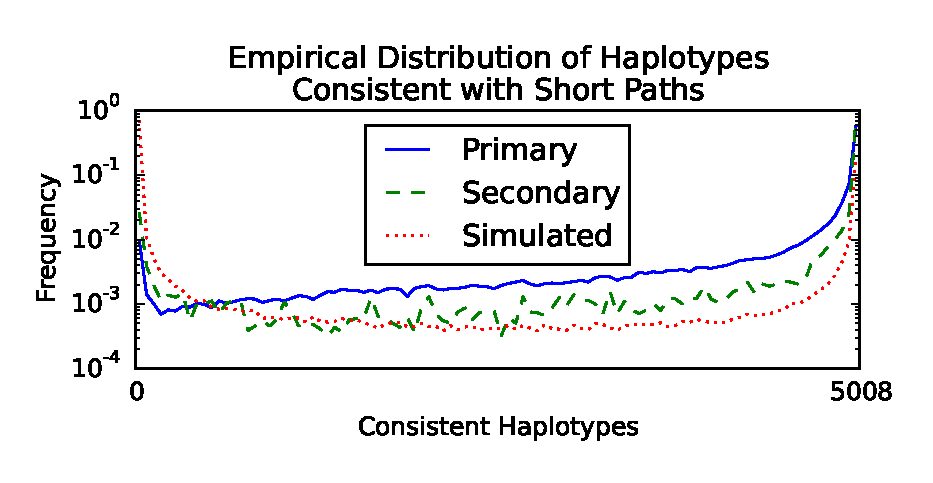
\includegraphics[width=\linewidth]{figures/03_gpbwt/histogram.eps}
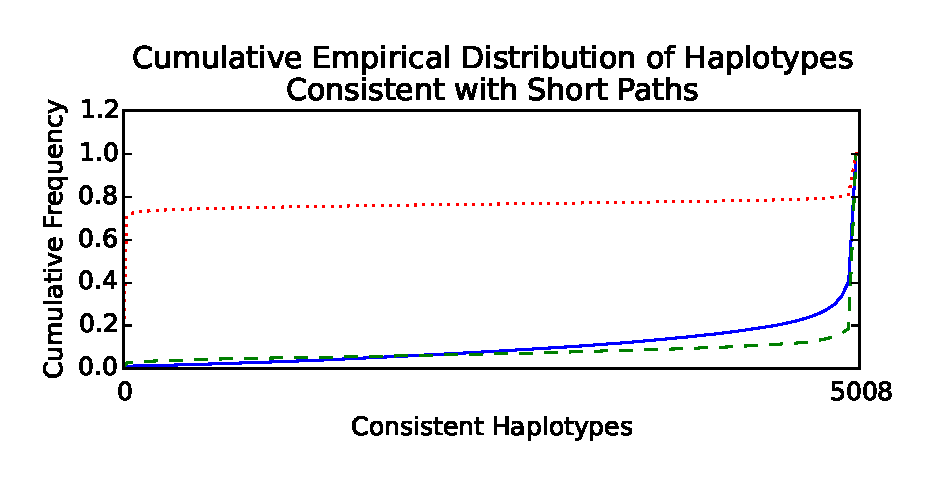
\includegraphics[width=\linewidth]{figures/03_gpbwt/cumulative.eps}
\caption{Distribution (top) and cumulative distribution (bottom) of the number of 1000~Genomes Phase 3 haplotypes consistent with short paths in the chromosome 22 graph. Primary mappings of 101~bp reads with scores of 90 out of 101 or above ($n=1,500,271$) are the solid blue line. Secondary mappings meeting the same score criteria ($n=43,791$) are the dashed green line. Simulated 100~bp random walks in the graph without consecutive \texttt{N} characters ($n=686,590$) are the dotted red line. Consistent haplotypes were counted using the gPBWT support added to \texttt{vg} \cite{garrison2016vg}.}
\label{fig:consistenthaplotypes}
\end{figure}


% Briefly describe implementation in xg and link to code
% Describe storing 1000-G haplotype data and give compression statistics

%Map Q scores with recombination
% TODO: MAPQ won't be done by the time we want to submit this, so I'm going to cut it - Adam

\subsection{Scaling Characteristics}

To evaluate the empirical space usage scaling characteristics of our gPBWT implementation, a scaling experiment was undertaken. The 1000 Genomes VCFs Phase 3 VCFs for the GRCh38 assembly were downloaded, modified to express all variants on the forward strand in the GRCh38 assembly, and used together with the assembly data to produce a graph for chromosome~22 based on the newer assembly. This graph was then used to construct a gPBWT with progressively larger subsets of the available samples. Samples were selected in the order they appear in the VCF file. For each subset, an \texttt{xg} serialization report was generated using the \texttt{xg} tool, and the number of bytes attributed to ``threads'' was recorded. The number of bytes used versus the number of samples stored is displayed in Figure \ref{fig:scaling}.

\begin{figure}[h!]
\centering
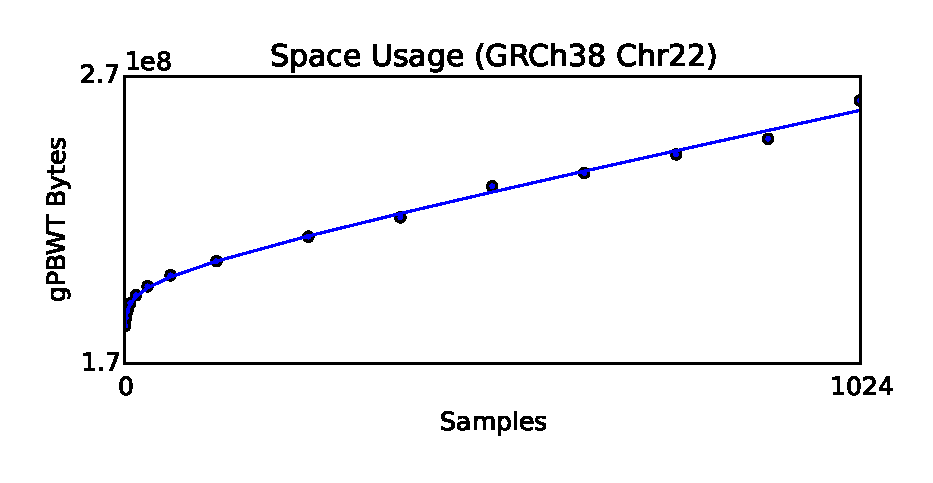
\includegraphics[width=\linewidth]{figures/03_gpbwt/scaling.eps}
\caption{Disk space usage for the gPBWT versus sample count for GRCh38 chromosome~22. Points are sampled at powers of two up to 128, and intervals of 128 thereafter up to 1024. The trend line shown corresponds to the function $y(x) = \num{3.16E6}~\mathrm{bytes} \cdot \ln(x / \mathrm{samples}) + \num{5.12E4}~\frac{\mathrm{bytes}}{\mathrm{sample}} \cdot x + \num{1.84E8}~\mathrm{bytes}$.}
\label{fig:scaling}
\end{figure}

After empirical size data was obtained, a log-plus-linear curve, consisting of a log component and a linear component, was fit to the data. This curve was used to extrapolate an estimated size of 5.34~GB on disk for the storage of 100,000 samples' worth of data on chromosome~22. We choose 100,000 because it is representative of the scale of large contemporary sequencing projects, such as Genomics England's 100,000 Genomes Project (\url{https://www.genomicsengland.co.uk/the-100000-genomes-project/}) \cite{nothaft2015rethinking} and the NHLBI's TOPMed program (\url{https://www.nhlbi.nih.gov/research/resources/nhlbi-precision-medicine-initiative/topmed}). Linear extrapolation from the 51~megabase chromosome~22 to the 3.2~gigabase human genome yields a size estimate of 336~GB for the storage of 100,000 diploid genomes, in addition to the space usage of the underlying graph. Although this extrapolation does not account for the dependence of graph complexity on the number of samples sequenced, it suggests that the gPBWT is capable of scaling to the anticipated size of future sequencing data sets, while using currently available computing resources.

\section{Discussion}

We have introduced the gPBWT, a graph based generalization of the PBWT. We have demonstrated that a gPBWT can be built for a substantial genome graph (all of human chromosome 22 and the associated chromosome 22 substitutions and indels in 1000~Genomes). Using this data structure, we have been able to quickly determine that the haplotype consistency rates of random walks and primary and secondary read mappings differ substantially from each other, and based on the observed distributions we hypothesize that consistency with very few haplotypes can be a symptom of a poor alignment. 

Such poor alignments could arise by a variety of means, including similarity between low complexity sequence, or paralogy; the latter representing true sequence homology but not true sequence orthology. Paralogous alignments are often difficult to distinguish from truly orthologous alignments, and can lead to the reporting of false or misplaced variants. Using haplotype consistency information is one way we might better detect paralogy, because paralogous sequence is not expected to be consistent with linkage relationships at a paralogous site. A more sophisticated analysis of haplotype consistency rate distributions could thus improve alignment scoring.

\begin{sloppypar}
In the present experiment, we have examined only relatively simple variation: substitutions and short indels. More complex variation, like large inversions and translocations, which would have induced cycles in our genome graphs, was both absent from the 1000 Genomes data set we used and unsupported by the optimized DAG-based construction algorithm which we implemented. We expect that complex structural variation is well suited to representation as a genome graph, so supporting it efficiently should be a priority for a serious practical gPBWT construction implementation.
\end{sloppypar}

\begin{sloppypar}
Extrapolating from our results on chromosome 22, we predict that a whole-genome gPBWT could be constructed for all 5,008 haplotypes of the 1000~Genomes data on GRCh37 and stored in the main memory of a reasonably apportioned computer, using about 27~GB of memory. On the GRCh38 data set, we extrapolate a space usage of 21~GB for the 2,504 samples of the 1,000~Genomes Project; A whole-genome gPBWT for 100,000~samples on GRCh38, we predict, could be stored in about 336~GB. Computers with this amount of memory, though expensive, are readily available from major cloud providers. The relatively modest growth from 5,008 haplotypes (2,504 samples) to 200,000 haplotypes (100,000 samples) is mostly attributable to the run-length compression used to store the $B$ arrays in our implementation. Each additional sample is representable as a mere increase in run lengths where it agrees with previous samples, and contributes a exponentially diminishing number of new variants and novel linkage patterns. While further empirical experimentation will be necessary to reasonably extrapolate further, it does not escape our notice that the observed scaling patterns imply the practicality of storing cohorts of a million or more individuals, such as those envisaged by the Precision Medicine Initiative \cite{hudson2015precision} and other similar national efforts, within an individual powerful computer. Looking forward, this combination of genome graph and gPBWT could potentially enable efficient mapping not just to one reference genome or collapsed genome graph, but simultaneously to an extremely large set of genomes related by a genome graph.
\end{sloppypar}

\section{List of Abbreviations}
\begin{itemize}
\item \textbf{BWT}: Burrows-Wheeler Transform
\item \textbf{PBWT}: Positional Burrows-Wheeler Transform
\item \textbf{gPBWT}: Graph Positional Burrows-Wheeler Transform
\item \textbf{GRC}: Genome Reference Consortium
\item \textbf{GRCh37}: GRC human genome assembly, build 37
\item \textbf{GRCh37}: GRC human genome assembly, build 38
\end{itemize}

\section{Declarations}

\subsection{Ethics approval and consent to participate}
All human data used in this study comes from already published, fully public sources, namely the 1000 Genomes Project and the human reference assembly. We believe that the work performed in this study is consistent with the purpose for which these data resources were created, and that the original ethical reviews of the creation and publication of these data resources, and the consent assertions given to the original projects, are sufficient to cover this new work.

\subsection{Consent for publication}
Not applicable

\subsection{Availability of data and material}
The datasets analyzed during the current study are available in the 1000 Genomes repository, at \url{ftp://ftp.1000genomes.ebi.ac.uk/vol1/ftp/release/20130502/ALL.chr22.phase3_shapeit2_mvncall_integrated_v5a.20130502.genotypes.vcf.gz} (md5 \texttt{ad7d6e0c05edafd7faed7601f7f3eaba}), \url{ftp://ftp.1000genomes.ebi.ac.uk/vol1/ftp/release/20130502/ALL.chr22.phase3_shapeit2_mvncall_integrated_v5a.20130502.genotypes.vcf.gz.tbi} (md5 4202e9a481aa8103b471531a96665047), \url{ftp://ftp.1000genomes.ebi.ac.uk/vol1/ftp/technical/reference/phase2_reference_assembly_sequence/hs37d5.fa.gz} (md5 \texttt{a07c7647c4f2e78977068e9a4a31af15}), and \url{ftp://ftp.1000genomes.ebi.ac.uk/vol1/ftp/release/20130502/supporting/GRCh38_positions/ALL.chr22.phase3_shapeit2_mvncall_integrated_v3plus_nounphased.rsID.genotypes.GRCh38_dbSNP_no_SVs.vcf.gz} (md5 \texttt{cf7254ef5bb6f850e3ae0b48741268b0}), and in the GRCh38 assembly repository, at \url{ftp://ftp.ncbi.nlm.nih.gov/genomes/all/GCA/000/001/405/GCA_000001405.15_GRCh38/GCA_000001405.15_GRCh38_assembly_structure/Primary_Assembly/assembled_chromosomes/FASTA/chr22.fna.gz} (md5 \texttt{915610f5fb9edfcc9ce477726b9e72c6}).

\section{Competing interests}
The authors declare that they have no competing interests.

\subsection{Funding}
This work was supported by the National Human Genome Research Institute of the National Institutes of Health under Award Number 5U54HG007990, the W.M. Keck foundation under DT06172015, the Simons Foundation under SFLIFE\# 351901, the ARCS Foundation, and Edward Schulak. The content is solely the responsibility of the authors and does not necessarily represent the official views of the National Institutes of Health or any other funder.

\section{Author's contributions}
    A.M.N. wrote most of the gPBWT implementation presented here, conducted the experiments, and composed the majority of the manuscript. E.G. managed the \texttt{vg} project, wrote the read simulation and mapping code used here, and collaborated on the gPBWT implementation. B.P. developed the mathematics of the gPBWT and collaborated on the manuscript.

\section{Acknowledgements}
We would like to thank Richard Durbin for inspiration and David Haussler for his extremely helpful comments on the manuscript.

